\section{Caution against a weak field approximation}
\label{appendix:continuum-time}

A weak field approximation for general relativistic effects is sometimes used in the interest of computational performance. For example, a spherical radius $R$ outside of which relativistic effects are said to be negligible, such that a flat (Minkowski) spacetime metric is used for ray-tracing and other calculations. In \citet{cackett_modelling_2014}, $R = 100\, \rg$ is used when calculating lag-frequency and lag-energy spectra. However, this approximation introduces a slight error when calculating the light travel time of flux from the disc and continuum source, which has a surprisingly significant effect on the computed lag-frequency spectra.

Since \Gradus is metric agnostic, we implement a new spacetime that switches to the Minkwoski form beyond $R$ and recalculate the lag-frequency relations. Our implementation preserves constant of motions across the boundary when switching from one metric to another, though other weak-field approximations may not, introducing additional errors in the trajectories of geodesics that depend on the ODE integration algorithm used and the solver steps over the boundary.

% The use of this weak-field approximation reproduces the results of \citet{cackett_modelling_2014}, but differs from the lag-frequency curve presented in this paper. We offer the following explanation:

% In cases where the source height above the black hole is small, the systematic error from the weak field approximation between the reflected and continuum flux is approximately equal, and therefore is negligible when the difference in arrival time is calculated, as in
% \begin{equation}
%     \Delta t = \tilde{t}_\text{reflected} - \tilde{t}_\text{continuum} ,
% \end{equation}
% where the tilde denotes the inclusion of some $\delta t$ due to the weak field approximation $\tilde{t} = t_\text{true} - \delta t$. However, when the source height is of appreciable value, say $h > 10\rg$, then for an off axis observer the systematic error introduced by $\delta t$ is greater for the continuum emission than for the reflected component (see Figure \ref{fig:app:weak-field-approx}), resulting in the continuum flux arriving seemingly too early. Note that $\delta t$ is dependant on the observer's position, and decreases with increasing $r_\text{obs}$.

% Figure \ref{fig:app:continuum-time} illustrates the relationship between coronal source height and $\delta t$, calculated by using the weak field approximation at different $R$ and subtracting the equivalent `true' light travel time $t$ (equivalent to $R \rightarrow \infty$). Even at $h = 100$, the continuum flux from the corona is seen to arrive significantly early.

% \begin{figure}
% 	\centering
% 	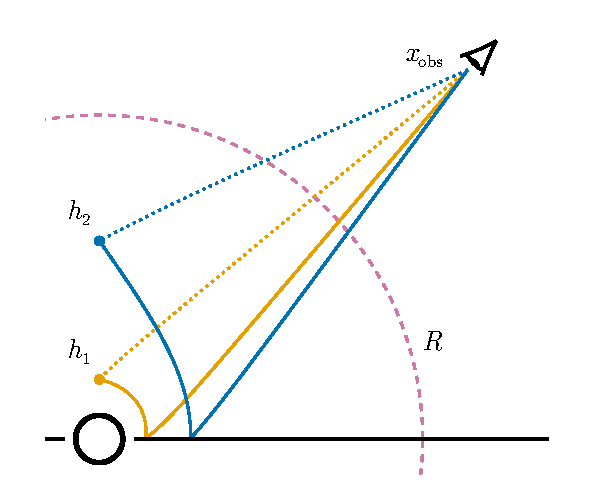
\includegraphics[width=0.80\linewidth]{figures/continuum-time.figure.pdf}
% 	\caption{\todo{TODO}}
% 	\label{fig:app:weak-field-approx}
% \end{figure}

% For the source heights of $h=10\, \rg$ and $h = 20 \rg$ and an observer inclination of $\theta_\text{obs} = 45^\circ$, the path length of the traject

% \todo{a heatmap showing $\delta t$ for different $h$ and observer distances?}

% \begin{figure}
% 	\centering
% 	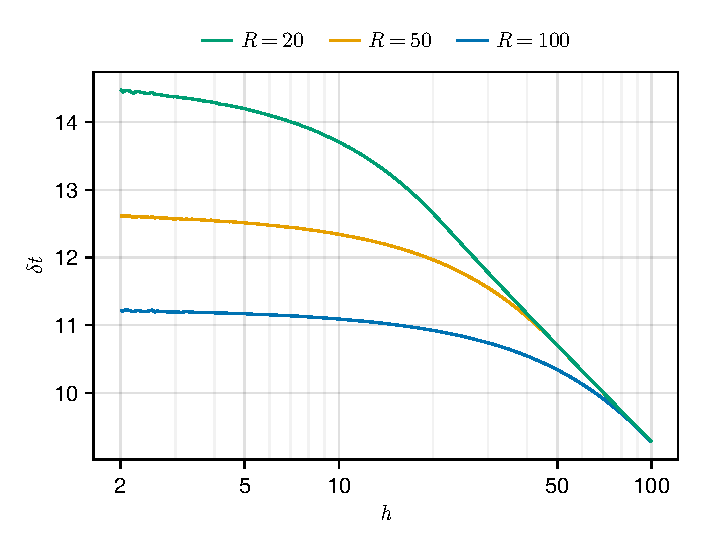
\includegraphics[width=0.98\linewidth]{figures/continuum-time.weak-field.pdf}
% 	\caption{\todo{TODO}}
% 	\label{fig:app:continuum-time}
% \end{figure}
